\documentclass[11pt]{exam}
\usepackage[margin=1in]{geometry}
\pagestyle{plain}
\usepackage{amsmath,amsfonts,amssymb,amsthm,enumerate}
\usepackage{multicol}
\usepackage[]{graphicx}
\usepackage{hyperref}
\usepackage{tikz}
\usepackage{pgfplots}
\usepackage{subfigure}
\usepackage[final]{pdfpages}

\addtolength{\footskip}{2\baselineskip} % to lower the page numbers
\title{\vspace{-1in} Math 115 Fall 2024 \\ Worksheet 15 -- MVT}
\date{}


% \theoremstyle{definition}
% \newtheorem{problem}{Problem}
\renewcommand{\questionlabel}{\textbf{Problem~\thequestion.}}
%\printanswers

\begin{document}
\maketitle
\vspace{-1in}

\section*{Warm-up questions}
\noindent
What are the hypothesis of the mean value theorem?

\vspace{3em}
\noindent
What is the conclusion of the mean value theorem?
\vspace{3em}
\begin{solution}
 Hypothesis
 \begin{itemize}
 \item \(f\) is continuous on \([a,b]\)
 \item \(f\) is differentiable on \((a,b)\)
 \end{itemize}
 Conclusion 
 \begin{itemize}
 \item There exists a number \(c\) with \(a < c < b\) such that \[
     f'(c) = \frac{f(b)-f(a)}{b-a} \,.
   \]
 \end{itemize}
\end{solution}
\begin{questions}
  \question Give an example of a function $f$ that is...
\begin{enumerate}[(a)]
	\item continuous on the interval $[-1,1]$ but that does not satisfy the hypothesis of the Mean Value Theorem on that interval, and for which the conclusion of the Mean Value Theorem is false.
	\item continuous on the interval $[-1,1]$ but that does not satisfy the hypothesis of the Mean Value Theorem on that interval, and for which the conclusion of the Mean Value Theorem is true.
	\item differentiable on the interval $(0,2)$ but that does not satisfy the hypothesis of the Mean Value Theorem on $[0,2]$.
\end{enumerate}
\begin{solution}
  \begin{enumerate}[(a)]
  \item \(f(x) = |x|\) on \(-1 \leq x \leq 1\).
  \item \[
      f(x) =
      \begin{cases}
        -x & -1 \leq x \leq 0\\
        2x & 0 < x \leq \frac{1}{2}\\
        3-4x & \frac{1}{2} < x \leq 1
      \end{cases}
    \]
  \item \[
      f(x) =
      \begin{cases}
        1 & x=0\\
        x^2 & 0 < x < 2\\
        0 & x=2
      \end{cases}
    \]
  \end{enumerate}
\end{solution}
\question (Winter 2018 Exam 2) The graph of the function $f$ with domain $-4 \leqslant x \leqslant 8$ is shown below. The function $f(x)$ satisfies:
\begin{itemize}
\item $f(x) = 1.5 x^{\frac{1}{3}}$ for $-1<x<1$, and
\item $f(x) = 4 +\displaystyle\sin \left( \frac{\pi}{4} (x-3) \right)$ for $3 \leqslant x < 5$ and $5 < x \leqslant 8$.
\end{itemize}
\vspace{-0.5em}
\begin{center}
  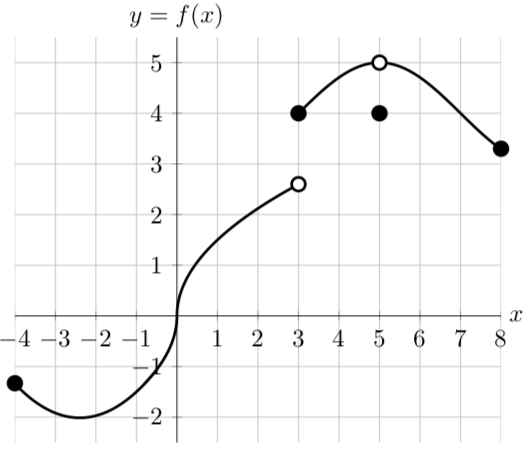
\includegraphics[scale=0.4]{Exam2W2018Problem5}
\end{center}

\begin{enumerate}[(a)]
	\item On which of the following intervals is the conclusion of the Mean Value Theorem true?
	$$[-4,0] \qquad [0,5] \qquad [1,3] \qquad [3,7] \qquad \textrm{none of these}$$
	\item On which of the following intervals are the hypothesis of the Mean Value Theorem true?
	$$[-4,0] \qquad [0,5] \qquad [1,3] \qquad [3,7] \qquad \textrm{none of these}$$
\end{enumerate}
\begin{solution}
  See \href{https://dhsp.math.lsa.umich.edu/exams/115exam2/w18/s5.pdf}{https://dhsp.math.lsa.umich.edu/exams/115exam2/w18/s5.pdf}
\end{solution}
\question (Fall 2017 Exam 2) Consider the graph of $h(x)$ below. Note that \(h\) is linear on the intervals $[-4,-1)$, $[-1,1]$ and $[1,2]$, differentiable on $(2, 5)$, and has a sharp corner at $x = 2$.
\begin{center}
  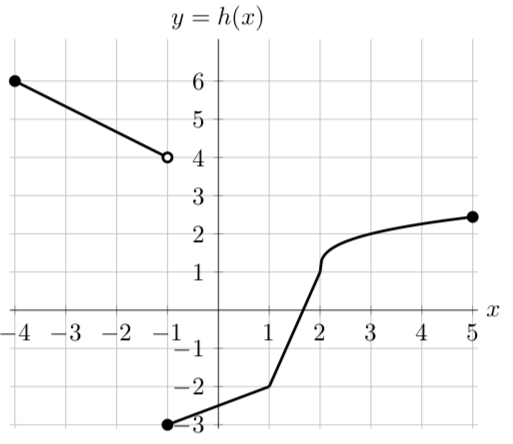
\includegraphics[scale=0.4]{Exam2Fall2017Problem4}
\end{center}
\begin{enumerate}[(a)]
	\item On which of the following intervals is the conclusion of the Mean Value Theorem true?
	$$[-4,-1] \qquad [-2,-1] \qquad [0,4] \qquad [2,5] \qquad \textrm{none of these}$$
	\item On which of the following intervals are the hypothesis of the Mean Value Theorem true?
	$$[-4,-1] \qquad [-2,-1] \qquad [0,4] \qquad [2,5] \qquad \textrm{none of these}$$
	\item For which values given below is the function $m(x) = h(h(x))$ not differentiable?
  Circle all that apply.
  $$x=-3 \qquad x=-1 \qquad x=2 \qquad x=3 \qquad x=4 \qquad \textrm{none of these}$$
	\end{enumerate}
        \begin{solution}
          See \href{https://dhsp.math.lsa.umich.edu/exams/115exam2/f17/s4.pdf}{https://dhsp.math.lsa.umich.edu/exams/115exam2/f17/s4.pdf}
        \end{solution}
\question The graph of a portion of the derivative of $b(x)$ is shown below. Assume that $b(x)$ is defined and continuous on $[-5, 6]$.
\begin{center}
  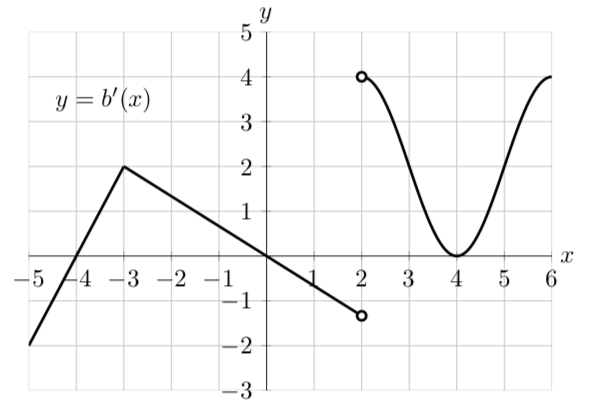
\includegraphics[scale=0.4]{Winter2017Exam2Problem1}
\end{center}
On which of the following intervals are the hypothesis of the Mean Value Theorem true?
		$$[-4,-2] \qquad [-2,2] \qquad [1,4] \qquad [-5,6] \qquad \textrm{none of these}$$
                \begin{solution}
                 See \href{https://dhsp.math.lsa.umich.edu/exams/115exam2/w17/s1.pdf}{https://dhsp.math.lsa.umich.edu/exams/115exam2/w17/s1.pdf}  
                \end{solution}
% \question (Fall 2016 Exam 2) The entire graph of a function $g(x)$ is shown below. Note that the graph of $g(x)$ has a horizontal tangent line at $x = 1$ and a sharp corner at $x = 4$.
% \begin{center}
%   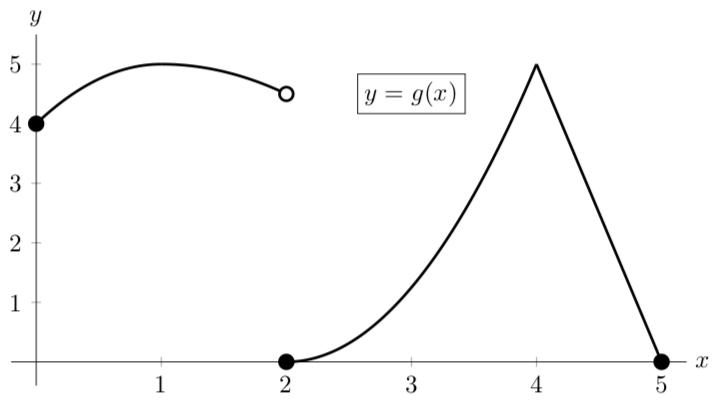
\includegraphics[scale=0.4]{Fall2016Exam2Problem6}
% \end{center}
% \begin{enumerate}[(a)]
% 		\item Let $L(x)$ be the local linearization of $g(x)$ near $x = 3$. Circle all the statements that are true.
% 		\begin{enumerate}[(1)]
% 		\begin{multicols}{3}
% 			\item $L(3) > g(3)$ 
% 			\item $L(3) = g(3)$ 
% 			\item $L(3) < g(3)$
% 			\item $L'(3) > g'(3)$ 
% 			\item $L'(3) = g'(3)$ 
% 			\item $L'(3) < g'(3)$
% 			\item $L(2.5) > g(2.5)$ 
% 			\item $L(2.5) = g(2.5)$ 
% 			\item $L(2.5) < g(2.5)$
% 			\item $L'(2.5) > g'(2.5)$ 
% 			\item $L'(2.5) = g'(2.5)$ 
% 			\item $L'(2.5) < g'(2.5)$
% 			\item $L(0) > g(0)$
% 			\item $L(0) = g(0)$ 
% 			\item $L(0) < g(0)$
% 			\item $L(5) > g(5)$ 
% 			\item $L(5) = g(5)$ 
% 			\item $L(5) < g(5)$
% 		\end{multicols}
% 		\centering \item None of these
% 		\end{enumerate}
		
% 		\item On which of the following intervals does $g$ satisfy the hypothesis of the Mean Value Theorem?
% 		$$[0,2] \qquad [0,4] \qquad [3,5] \qquad [4,5] \qquad \textrm{none of these}$$
% 		\item  On which of the following intervals does $g$ satisfy the conclusion of the Mean Value Theorem?
% 		$$[0,2] \qquad [0,4] \qquad [3,5] \qquad [4,5] \qquad \textrm{none of these}$$
% 	\end{enumerate}

                \question (Fall 2016 Exam 2)
The entire graph of a function \(g(x)\) is shown below. Note that the graph of \(g(x)\)
has a horizontal tangent line at \(x = 1\) and a sharp corner at \(x = 4\).
\begin{center}
  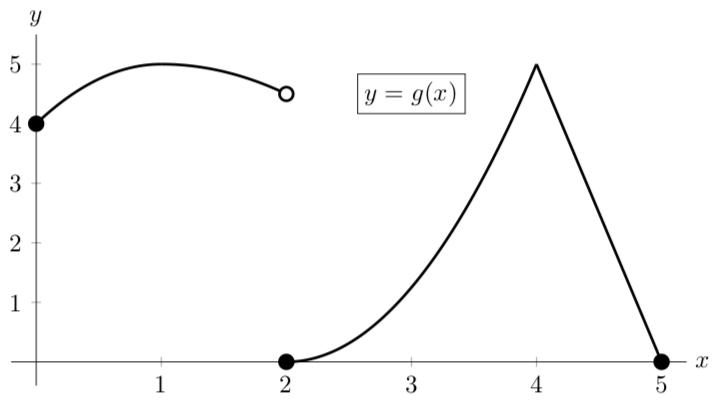
\includegraphics[scale=0.4]{Fall2016Exam2Problem6}
\end{center}
\begin{enumerate}[(a)]
\item On which of the following intervals does the function \(f(x)\) satisfy the hypotheses of
  the Mean Value Theorem? Circle the correct answer(s): \[
[0,2] \qquad [1,3] \qquad [2,4] \qquad [3,5] \qquad \textrm{None of these}
  \]
\item On the interval \([8, 12]\) the hypotheses of the Mean Value Theorem are true for the
function f(x). What does the conclusion of this theorem say in this interval?\\
{\bf Answer:}
\vspace{0.5in}
\end{enumerate}
\begin{solution}
  See \href{https://dhsp.math.lsa.umich.edu/exams/115exam2/f16/s6.pdf}{https://dhsp.math.lsa.umich.edu/exams/115exam2/f16/s6.pdf}
\end{solution}
\question (Winter 2016 Exam 2) Let $h(x)$ be a twice differentiable function defined for all real numbers $x$. (So $h$ is differentiable and its derivative $h'$ is also differentiable.)
Some values of the derivative of $h$ are given in the table below.
\begin{center}
  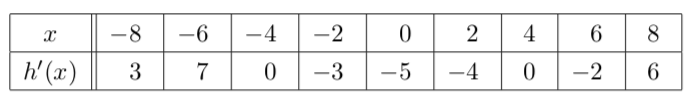
\includegraphics[scale=0.5]{Winter2016Exam2Problem4}
\end{center}

\begin{enumerate}[(a)]
\item Circle all the intervals which must contain a number $c$ such that $h''(c)=2$.
$$-8 < x < -6 \qquad -4 < x < -2 \qquad -2 < x < 0 \qquad 6 < x < 8$$
\item Suppose that $h''(x)<0$ for $x<-8$ and $h(-8)=7$. Circle all the numbers below which could equal the value of $h(-10)$.
$$-2 \qquad -1 \qquad 0 \qquad 1 \qquad 2  \qquad \textrm{None of these}$$
\end{enumerate}
\begin{solution}
  See \href{https://dhsp.math.lsa.umich.edu/exams/115exam2/w16/s4.pdf}{https://dhsp.math.lsa.umich.edu/exams/115exam2/w16/s4.pdf} 
\end{solution}
\end{questions}
\end{document}

%%% Local Variables:
%%% mode: latex
%%% TeX-master: t
%%% End:
